\documentclass[tikz, border=5mm]{standalone}
\usepackage{pgfplots}
\pgfplotsset{compat=1.18}

\begin{document}
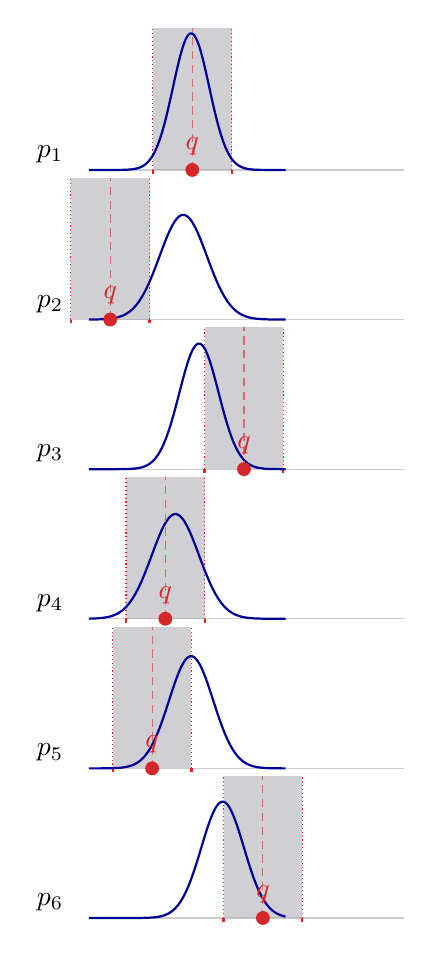
\begin{tikzpicture}[
    % Definición de función gaussiana estándar
    declare function={gauss(\x,\mu,\sigma)=1/(\sigma*sqrt(2*pi))*exp(-((\x-\mu)^2)/(2*\sigma^2));},
    % Estilo para las curvas
    gaussian plot/.style={
        thick, color=blue!60!black, smooth,
        domain=0:2.5, samples=100
    }
]
    % Configuración de colores
    \definecolor{bandgrey}{RGB}{160, 160, 170}
    \definecolor{pointqred}{RGB}{214, 39, 40}

    % Parámetros generales
    \def\verticaloffset{1.9} % Espaciado vertical entre cascadas
    \def\qr{0.5} % Radio 'r' para el intervalo

    % Fijar semilla para que las posiciones aleatorias sean reproducibles
    \pgfmathsetseed{2026}

    % Bucle para generar las 8 gaussianas
    % Parámetros: {índice / media / desviación estándar}
    % qx ahora se calcula dinámicamente dentro del bucle
    \foreach \i/\mu/\sigma in {
        1/1.3/0.23,
        2/1.2/0.3,
        3/1.4/0.25,
        4/1.1/0.3,
        5/1.3/0.28,
        6/1.7/0.27
    }{
        % Cálculo del desplazamiento vertical
        \pgfmathsetmacro{\yshift}{(6-\i)*\verticaloffset}

        % Generar una posición aleatoria para q 
        % 'rnd' produce un valor entre 0 y 1
        \pgfmathsetmacro{\qx}{\mu + (rnd-0.5)*2} % q se distribuye alrededor de la media

        % Línea de base horizontal
        \draw[thin, black!20] (0,\yshift) -- (4,\yshift);

        % Leyenda de la gaussiana (p_i)
        \node [anchor=east, font=\bfseries] at (-0.2, {0.2 + \yshift}) {$p_{\i}$};

        % 1. Dibujar el rango de consulta como una "ventana" translúcida alta
        \fill[bandgrey, opacity=0.5] (\qx-\qr, \yshift) rectangle (\qx+\qr, \yshift + 1.8);
        
        % Bordes verticales para delimitar el intervalo
        \draw[thin, red!90, densely dotted] (\qx-\qr, \yshift) -- (\qx-\qr, \yshift + 1.8);
        \draw[thin, red!90, densely dotted] (\qx+\qr, \yshift) -- (\qx+\qr, \yshift + 1.8);

        % Marcas del intervalo en la base
        \draw[thick, red!90] (\qx-\qr, \yshift) -- (\qx-\qr, \yshift-0.05);
        \draw[thick, red!90] (\qx+\qr, \yshift) -- (\qx+\qr, \yshift-0.05);

        % 2. Trazado de la curva gaussiana
        \draw [gaussian plot] plot (\x, {gauss(\x,\mu,\sigma) + \yshift});

        % 3. Proyectar el punto q sobre la curva
        \pgfmathsetmacro{\qy}{gauss(\qx,\mu,\sigma) + \yshift}
        
        % Línea desde el eje X hasta el punto en la curva
        \draw[densely dashed, pointqred!70] (\qx, \yshift) -- (\qx, \yshift + 1.8);
        
        % Punto q marcado en rojo sobre la gaussiana
        \fill [pointqred] (\qx, \yshift) circle (2.5pt) node[above=2pt, font=\bfseries] {$q$};
    }

\end{tikzpicture}
\end{document}
